\section*{Exercice 189 -- SLCI -- Numérique}
\setcounter{exo}{0}
%CCS PSI 2015


\begin{obj}
Compléter la loi de commande afin de limiter la sensibilité du système aux bruits de mesure.
\end{obj}

Le moteur retenu possède les caractéristiques suivantes : tension nominale de \SI{42}{V}, couple maximal en fonctionnement
de \SI{113}{mN.m}. De plus, lorsque la vitesse de rotation de l’arbre moteur est nulle, pour des raisons
techniques, la valeur absolue du couple moteur ne doit pas excéder \SI{10}{\%} du couple maximal, soit \SI{11,3}{mN.m} en réponse aux sollicitations dues aux bruits de mesure.
Le dimensionnement de la loi de commande effectué à la partie précédente ne prend pas en compte tous les
phénomènes indésirables susceptibles de dégrader les performances du système étudié. L’un d’entre eux est le
bruit de mesure du capteur de position angulaire des axes moteurs. Le signal brut issu du capteur est de nature
analogique. Pour qu’il soit exploitable par le calculateur, ce signal est numérisé. On obtient alors une image de
la position sous la forme d’un ensemble de points. On note $T_e$ la période d’échantillonnage.
On note $f_k$, $k\in\mathbb{N}$ la valeur d’une fonction continue $f(t)$ prise au k\ieme échantillonnage, c’est-à-dire que
$f_k=f\left(kT_e\right)$. En sortie du convertisseur analogique/numérique, seules les valeurs $f_k$ pour $k$ entier sont disponibles.
Pour l’axe 1, $\Delta \theta_1(t)=$ est l’angle en sortie du moteur et $s_k$ est la grandeur numérisée de la position angulaire
mesurée.
L’imperfection de la chaîne de mesure implique la présence d’une composante aléatoire sur chaque valeur de $s_k$
image de l’angle $\delta \theta_1(t)$, en plus de la composante non aléatoire. Chaque valeur $s_k$ peut donc se décomposer
sous la forme d’une somme d’une composante non aléatoire notée $s_k^b$, de variance
$\text{var}\left( s_k^b\right)$ identique pour tout $k$. De plus, $s_{k-1}^b$ sont des variables aléatoires indépendantes.


La loi de commande (II.2) est, en pratique, réalisée numériquement. Sa discrétisation conduit à la forme suivante :
$$
u_{1k} = \sigma_1 \cdot\left(s_{ck}-s_k \right)+\sigma_2 \cdot h\left(s_{ck}-s_k \right)  -\sigma_3 g \left(s_k \right) + \sigma_4 s_{ck}.
$$

avec
\begin{itemize}
\item $s_{ck}$ la valeur au k\ieme instant de l’image de la consigne ;
\item $h\left(s_{ck}-s_k \right)$ une fonction permettant d’approcher l’intégrale d’une grandeur numérique ;
\item $g\left(s_{ck}\right)$ une fonction permettant d’approcher la dérivée d’une grandeur numérique ;
\item $u_{1k}$ la tension de commande du moteur prise au k\ieme instant.
\end{itemize}
Le schéma fonctionnel pour la prise en compte des bruits de mesure est donné figure 10. Pour simplifier, la
perturbation due à la réaction du tissu humain sur l’outil n’est pas prise en compte. On suppose que le CNA
(Convertisseur Numérique Analogique) n’a pas d’influence sur l’étude menée.

\begin{center}

%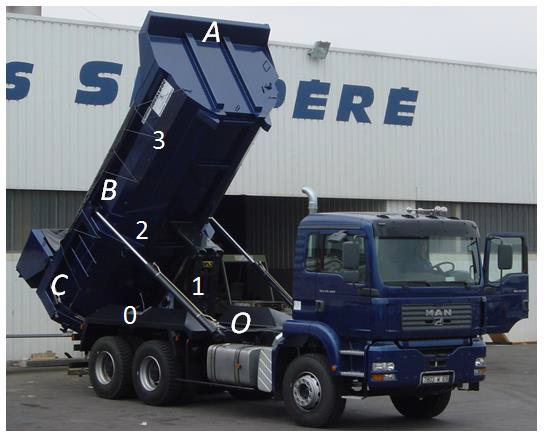
\includegraphics[width=\linewidth]{996_01}

\textit{Modèle utilisé pour la simulation}
\end{center}


Ainsi, une simulation a été réalisée pour une consigne en échelon de position nulle $(\forall k \in \mathbb{N}, s_{ck}=0)$
pour visualiser l’impact du bruit de mesure de l’axe 1. De plus, chaque terme $s_k^b$
est modélisé par une variable aléatoire suivant une loi normale de moyenne nulle et d’écart type $\SI{3,3e-4}{rad}$, soit une variance de $\SI{1,1e-7}{rad^2}$. La période d’échantillonnage est $T_e = \SI{100}{\mu s}$.


\begin{center}

%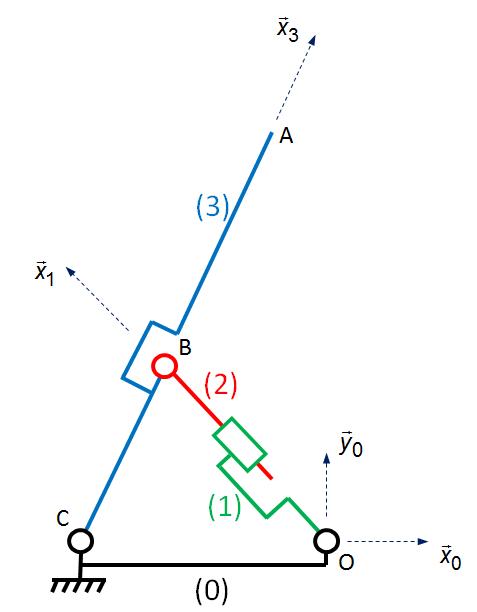
\includegraphics[width=\linewidth]{996_02}

\textit{Résultats de la simulation, impact du bruit de mesure}
\end{center}



\subparagraph{}
\textit{En justifiant, expliquer pourquoi il est nécessaire de filtrer le bruit de mesure en observant les courbes
de tension de commande, puis du couple moteur.}
\ifprof
\begin{corrige}
\end{corrige}
\else
\fi


\subparagraph{}
\textit{En observant la courbe représentative de $\Delta\theta_1(t)$ de la figure 11, justifier pourquoi les imperfections de
la chaîne de mesure n’influencent pas la position angulaire $\Delta\theta_1(t)$.}
\ifprof
\begin{corrige}
\end{corrige}
\else
\fi


\subparagraph{}
\textit{En utilisant les équations du moteur (II.1) et en se plaçant à un point de fonctionnement stabilisé,
c’est-à-dire à vitesse nulle, déterminer la valeur numérique maximale (en valeur absolue) de la tension à ne pas
dépasser pour que le couple n’excède pas \SI{11,3}{mN.m} en valeur absolue.}
\ifprof
\begin{corrige}
\end{corrige}
\else
\fi

Afin de limiter les effets néfastes du bruit de mesure sur le système, un filtre numérique est intégré dans la
chaine de mesure, cf figure 12.


\begin{center}

%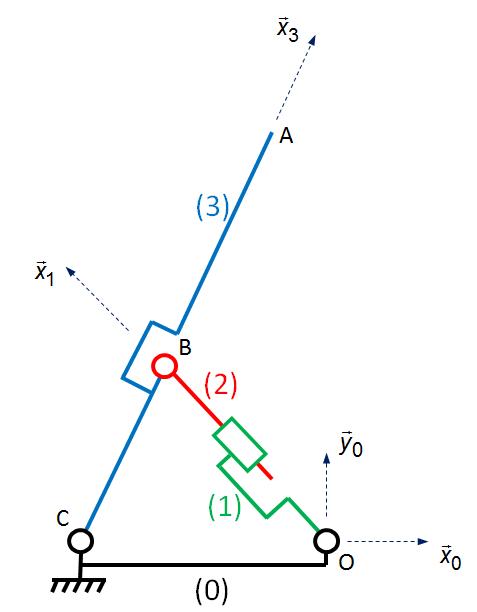
\includegraphics[width=\linewidth]{996_02}

\textit{Intégration du filtre numérique}
\end{center}

On note $s_k^f$ la valeur filtrée au k\ieme instant. L’objectif de l’étude qui suit est de limiter la variation de
tension engendrée par le bruit de mesure en dimensionnant le filtre. Seul l’impact du bruit est étudié, donc on
considère la consigne de position nulle, et au vu des résultats de simulation, on fera dans ce cas l’hypothèse que
$\Delta\theta_1(t)=\SI{0}{rad}$, ce qui implique $\forall k \in \mathbb{N}, s_k^a =0$.
La question précédente a permis de déterminer une valeur absolue maximale de la tension à ne pas dépasser. On admettra
que ce résultat impose alors une variance maximale de $\SI{0,02}{V^2}$ pour $u_{1k}$.
Le filtre numérique retenu est l’équivalent d’un filtre passe-bas analogique du premier ordre, de constante de
temps $T_f$ et de gain statique unitaire.

\subparagraph{}
\textit{Dans le cas d’une réalisation analogique du filtre, donner la relation entre $s^f(t)$, $s(t)$ et $T_f$, sous la
forme d’une équation différentielle. En déduire l’expression de $s_k^f$ en fonction de 
$s_k$, $s_{k-1}^f$, $T_f$ et $T_e$ dans le cas d'une réalisation numérique. On retiendra la formule suivante pour la dérivée discrète correspondant à la dérivée continue d’une fonction temporelle $f(t)$ à l’instant $t=kT_e$ : 
$\dfrac{f_k  -f_{k-1}}{T_e}$ où $T_e$ est la période d’échantillonnage.}

\ifprof
\begin{corrige}
\end{corrige}
\else
\fi

On rappelle que si $x$ et $y$ sont des variables aléatoires de variance $\text{var}(x)$ et $\text{var}(y)$ respectivement, $a$ et $b$ des nombres réels, alors on a : $\text{var}\left(ax+b\right) = a^2 \text{var}(x)$ $\text{var}\left(x+y\right) = \text{var}(x)+\text{var}(y)+2\text{cov}(x,y)$. 

Si les deux variables aléatoires sont indépendantes, alors $\text{cov}(x,y)=0$.
L’estimation de la variance du signal filtré, notée $\text{var}\left(s_k^f\right)$, est nécessaire pour dimensionner le filtre. Plusieurs centaines de simulations ont montré que l’évolution de $\text{var}\left(s_k^f\right)$ en fonction de $k$ reste similaire à celle montrée à
la figure 13. Pour un nombre d’échantillons suffisamment important, la variance devient constante et sa valeur
dépend de $T_f$.

\begin{center}
\centering
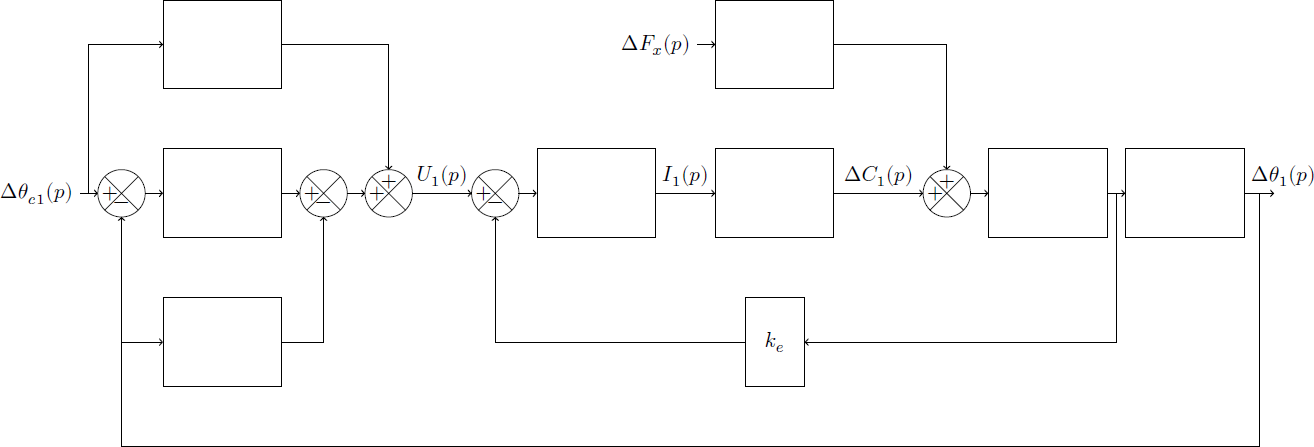
\includegraphics[width=\linewidth]{997_01}
\end{center}

\subparagraph{}
\textit{Quelle approximation peut-on faire concernant $\text{var}\left(s_k^f\right)$ et $\text{var}\left(s_{k-1}^f\right)$ ? Justifier la réponse.}
\ifprof
\begin{corrige}
\end{corrige}
\else
\fi


\subparagraph{}
\textit{Exprimer alors $\text{var}\left(s_k^f\right)$ en fonction de  $\text{var}\left(s_{k}\right)$, $T_f$ et $T_e$.}
\ifprof
\begin{corrige}
\end{corrige}
\else
\fi


On admettra que la relation entre $\text{var}\left(s_k^f\right)$ et $\text{var}\left(u_{1k}\right)$
en utilisant la loi de commande avec les paramètres du correcteur dimensionné dans la partie précédente est, pour tout $k$, 
$\text{var}\left(u_{1k}\right)=n_0 \text{var}\left(s_{k}^f\right)$ avec $n_0=6337147$.


\subparagraph{}
\textit{Donner l’expression littérale de $T_f$, puis calculer sa valeur en secondes qui permet d’assurer une variance
du signal de commande $\text{var}\left(u_{1k}\right) \leq \SI{0,02}{V^2}$. On rappelle les valeurs suivantes : 
$\text{var}\left(s_{k}\right) =\SI{1,1e-7}{rad^2}$, $T_e = \SI{1e-4}{s}$.}
\ifprof
\begin{corrige}
\end{corrige}
\else
\fi



%\begin{center}
%\centering
%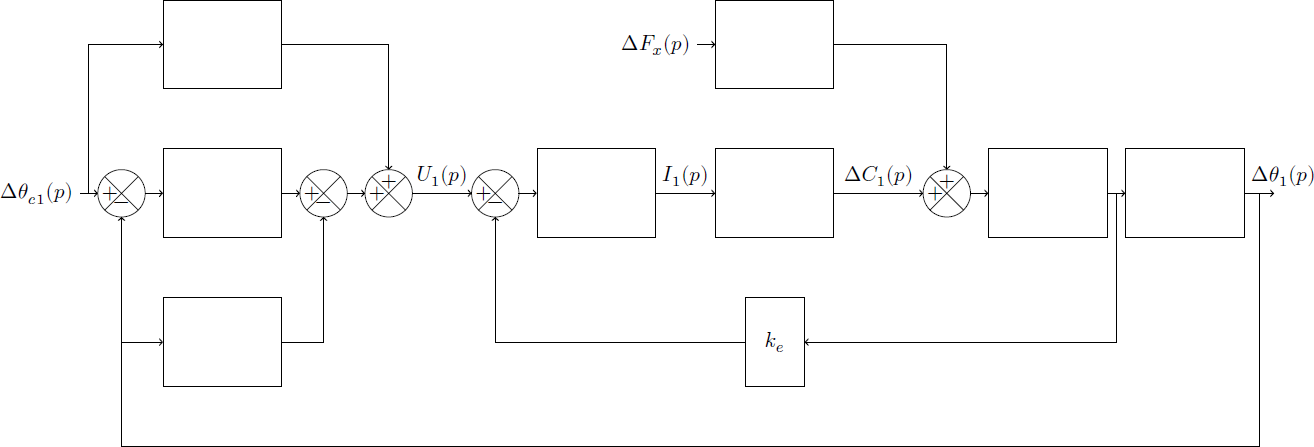
\includegraphics[width=\linewidth]{997_01}
%\end{center}


%
%\begin{figure}%[H]
%\centering
%\rotatebox{90}{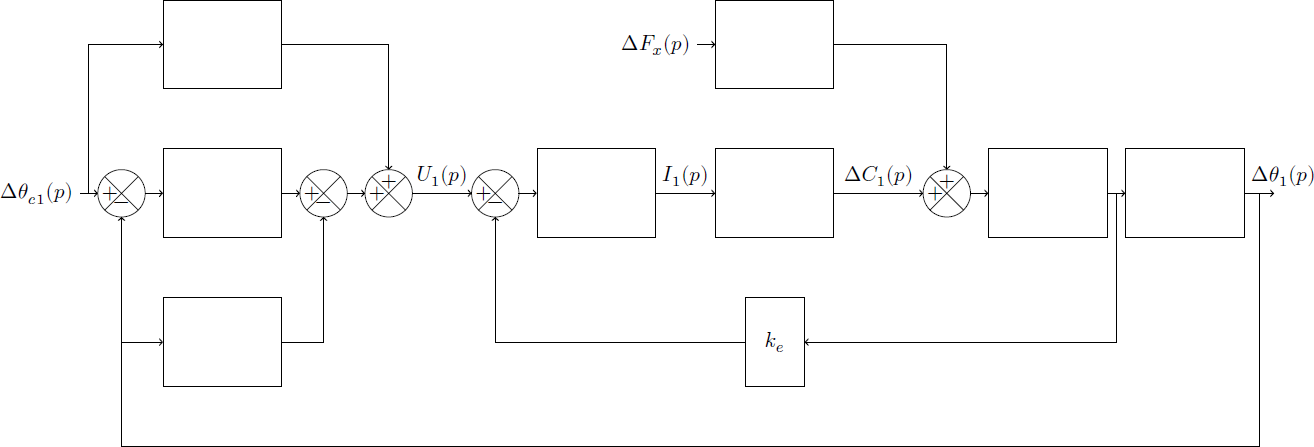
\includegraphics[height=\linewidth]{997_01}}
%
%%\label{fig_2_5}
%%\caption{Schéma cinématique du modèle mécanique adopté}
%\end{figure}
%
